\documentclass[10pt, letterpaper]{article}
\usepackage[utf8]{inputenc}
\usepackage{amsmath}
\usepackage{amssymb}
\usepackage{bbm}
\usepackage{booktabs}
\usepackage{caption}
\usepackage{color}
\usepackage[shortlabels]{enumitem}
\usepackage{fancyhdr}
\usepackage{hyperref}
\usepackage{geometry}
\geometry{a4paper,scale=0.8}
\usepackage{graphicx}
\graphicspath{ {./img/}}
\usepackage{listings}
\usepackage{mathtools}
\usepackage{mathrsfs}
\usepackage{setspace}
\usepackage{subfigure}
\renewcommand{\baselinestretch}{1.3}

% set-up header & footer
\pagestyle{empty}
\fancyhf{}
\cfoot{\thepage}
\lhead{%
\textbf{University of California, Berkeley} \\
Department of Civil \& Environ. Eng.
}
\rhead{\textbf{CS 285 Deep Reinforcement Learning}\\\date{\today}}

\title{%
    \textbf{Homework 4}
}
\author{Juanwu Lu (3037432593)\\ \small(M.Sc. Civil Engineering, UC Berkeley)}
\date{}

% set-up code listing
\definecolor{dkgreen}{rgb}{0,0.6,0}
\definecolor{gray}{rgb}{0.5,0.5,0.5}
\definecolor{manuve}{rgb}{0.58,0,0.82}

\lstset{frame=tb,
    language=Python,
    aboveskip=3mm,
    belowskip=3mm,
    showstringspaces=false,
    columns=flexible,
    basicstyle={\small\ttfamily},
    numbers=none,
    numberstyle=\tiny\color{gray},
    keywordstyle=\color{blue},
    commentstyle=\color{dkgreen},
    stringstyle=\color{manuve},
    breaklines=true,
    breakatwhitespace=true,
    tabsize=3
}

\begin{document}
\maketitle
\captionsetup[figure]{labelfont={bf},labelformat={default},labelsep=period,name={Figure}}
\captionsetup[table]{labelfont={bf},labelformat={default},labelsep=period,name={TABLE}}
\thispagestyle{fancy}
\pagestyle{plain}

% Problem 1
\section*{Problem 1}

\begin{figure}[thbp]
    \subfigure[]{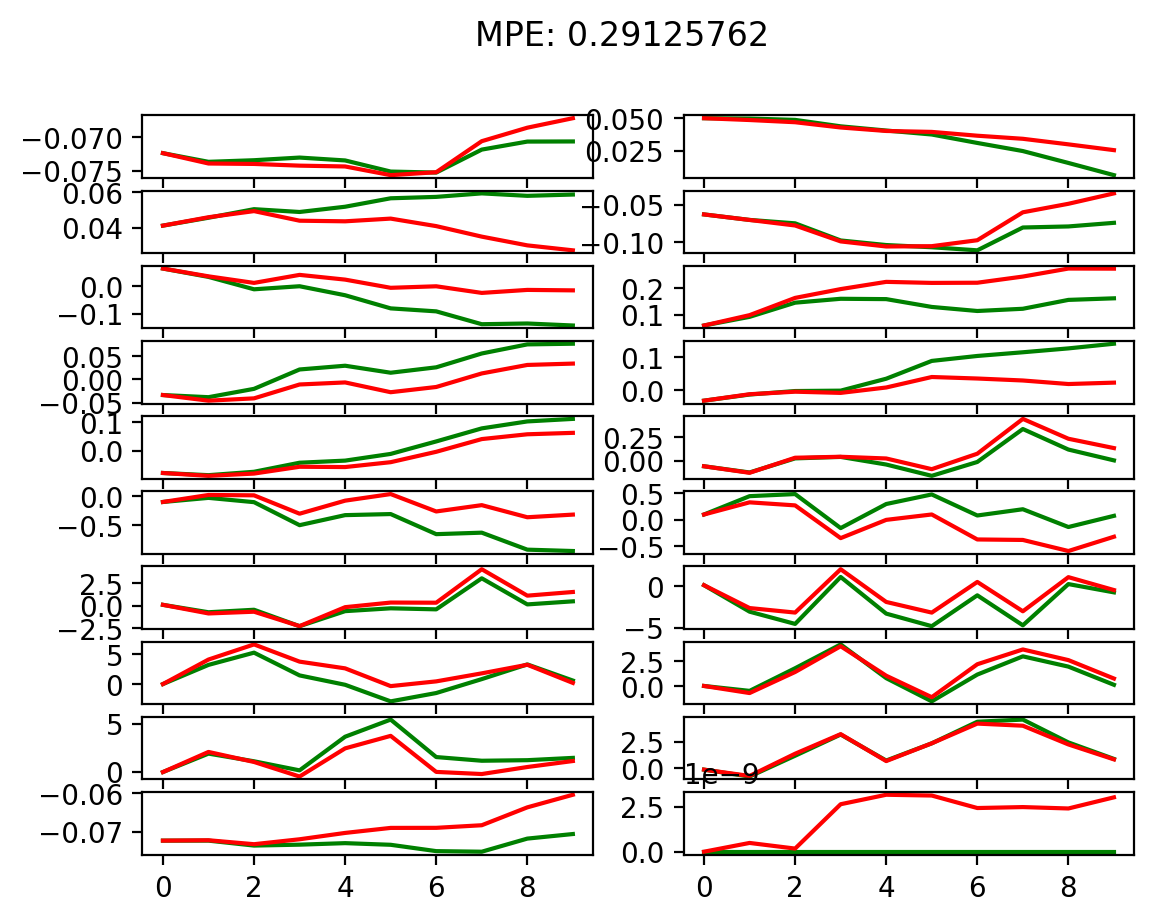
\includegraphics[width=0.3\textwidth]{q1_n500_a132.png}}
    \subfigure[]{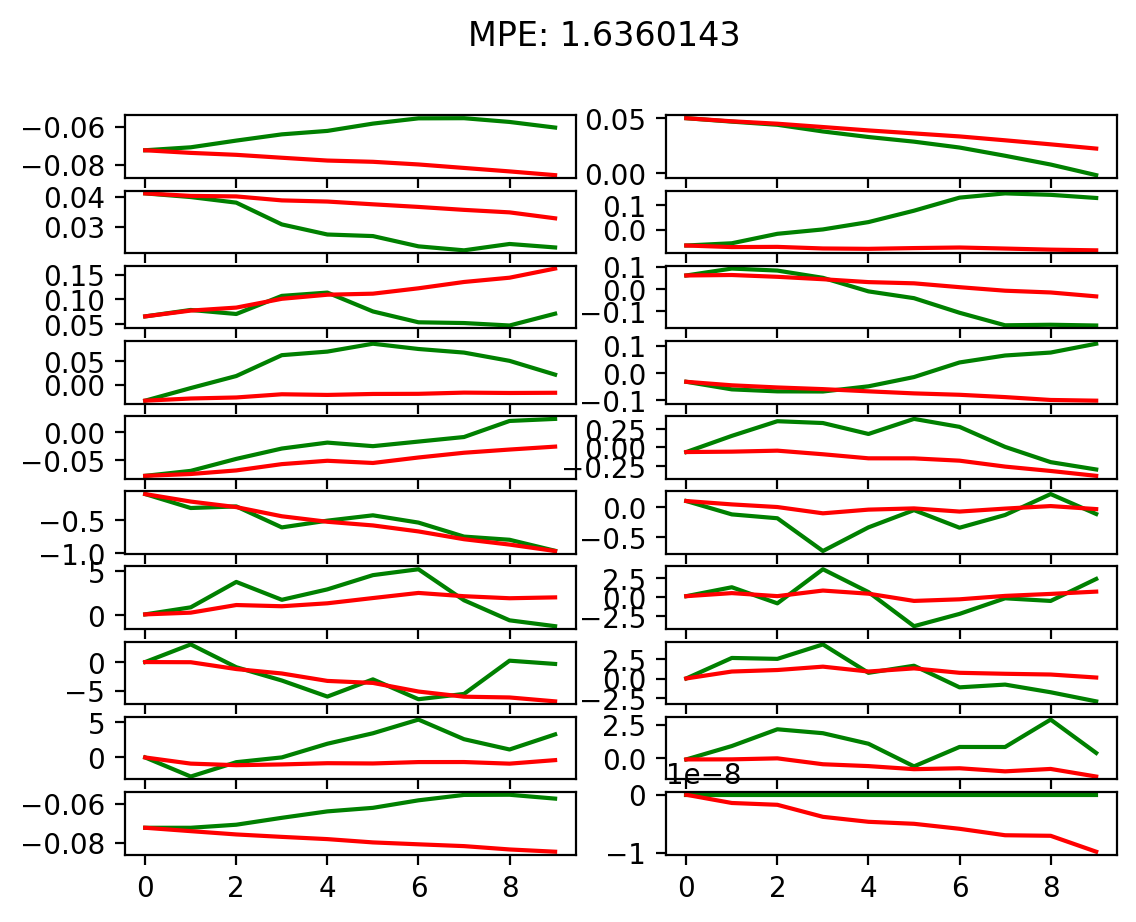
\includegraphics[width=0.3\textwidth]{q1_n5_a2250.png}}
    \subfigure[]{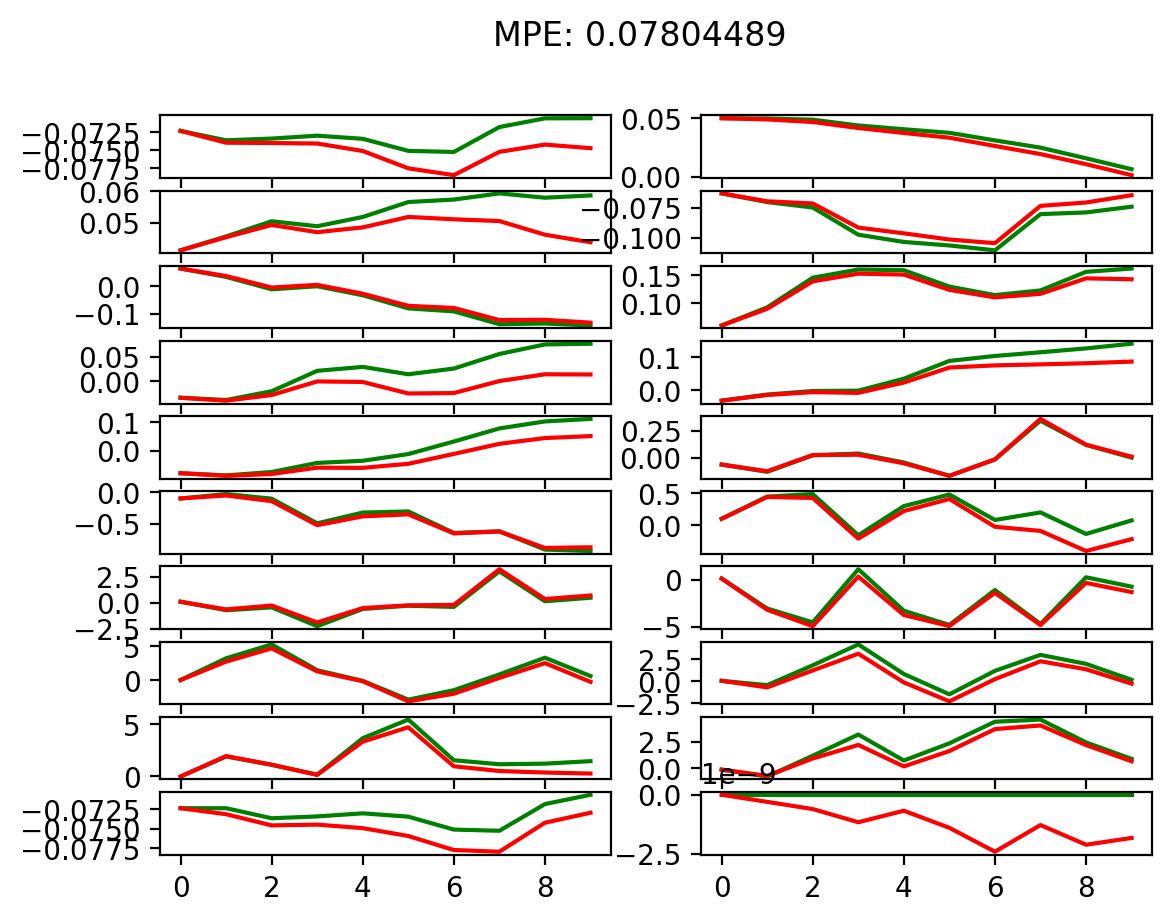
\includegraphics[width=0.3\textwidth]{q1_n500_a2250.png}}
    \caption{Results from different settings: (a) 1 hidden layer, 32 neurons, 500 steps; (b) 2 hidden layers, 250 neurons, 5 steps; (c) 2 hidden layers, 250 neurons, 500 steps.}
    \label{fig:1}
\end{figure}

Based on the results in \hyperref[fig:1]{Figure 1}, training with a neural network consisting of two hidden layers of 250 neurons with 500 agent training steps each iteration achieves the best performance (i.e., with the lowewst MPE). Meanwhile, by comparing figure 1(b) and 1(c), I can tell that increasing the number of agent training steps per iteration has more significant improvement on the final performance than increasing the complexity of the neural network model.

\begin{lstlisting}
    echo "Running Homework 4 Problem 1";
    python cs285/scripts/run_hw4_mb.py --exp_name q1_cheetah_n500_arch1x32 --env_name cheetah-cs285-v0 --add_sl_noise --n_iter 1 --batch_size_initial 20000 --num_agent_train_steps_per_iter 500 --n_layers 1 --size 32 --scalar_log_freq -1 --video_log_freq -1 --mpc_action_sampling_strategy random -gpu_id $1 &
    python cs285/scripts/run_hw4_mb.py --exp_name q1_cheetah_n5_arch2x250 --env_name cheetah-cs285-v0 --add_sl_noise --n_iter 1 --batch_size_initial 20000 --num_agent_train_steps_per_iter 5 --n_layers 2 --size 250 --scalar_log_freq -1 --video_log_freq -1 --mpc_action_sampling_strategy random -gpu_id $1 &
    python cs285/scripts/run_hw4_mb.py --exp_name q1_cheetah_n500_arch2x250 --env_name cheetah-cs285-v0 --add_sl_noise --n_iter 1 --batch_size_initial 20000 --num_agent_train_steps_per_iter 500 --n_layers 2 --size 250 --scalar_log_freq -1 --video_log_freq -1 --mpc_action_sampling_strategy random -gpu_id $1 &
    wait;
    echo "Done";
\end{lstlisting}

\pagebreak
% Problem 2
\section*{Problem 2}

\begin{figure}[thbp]
    \centering
    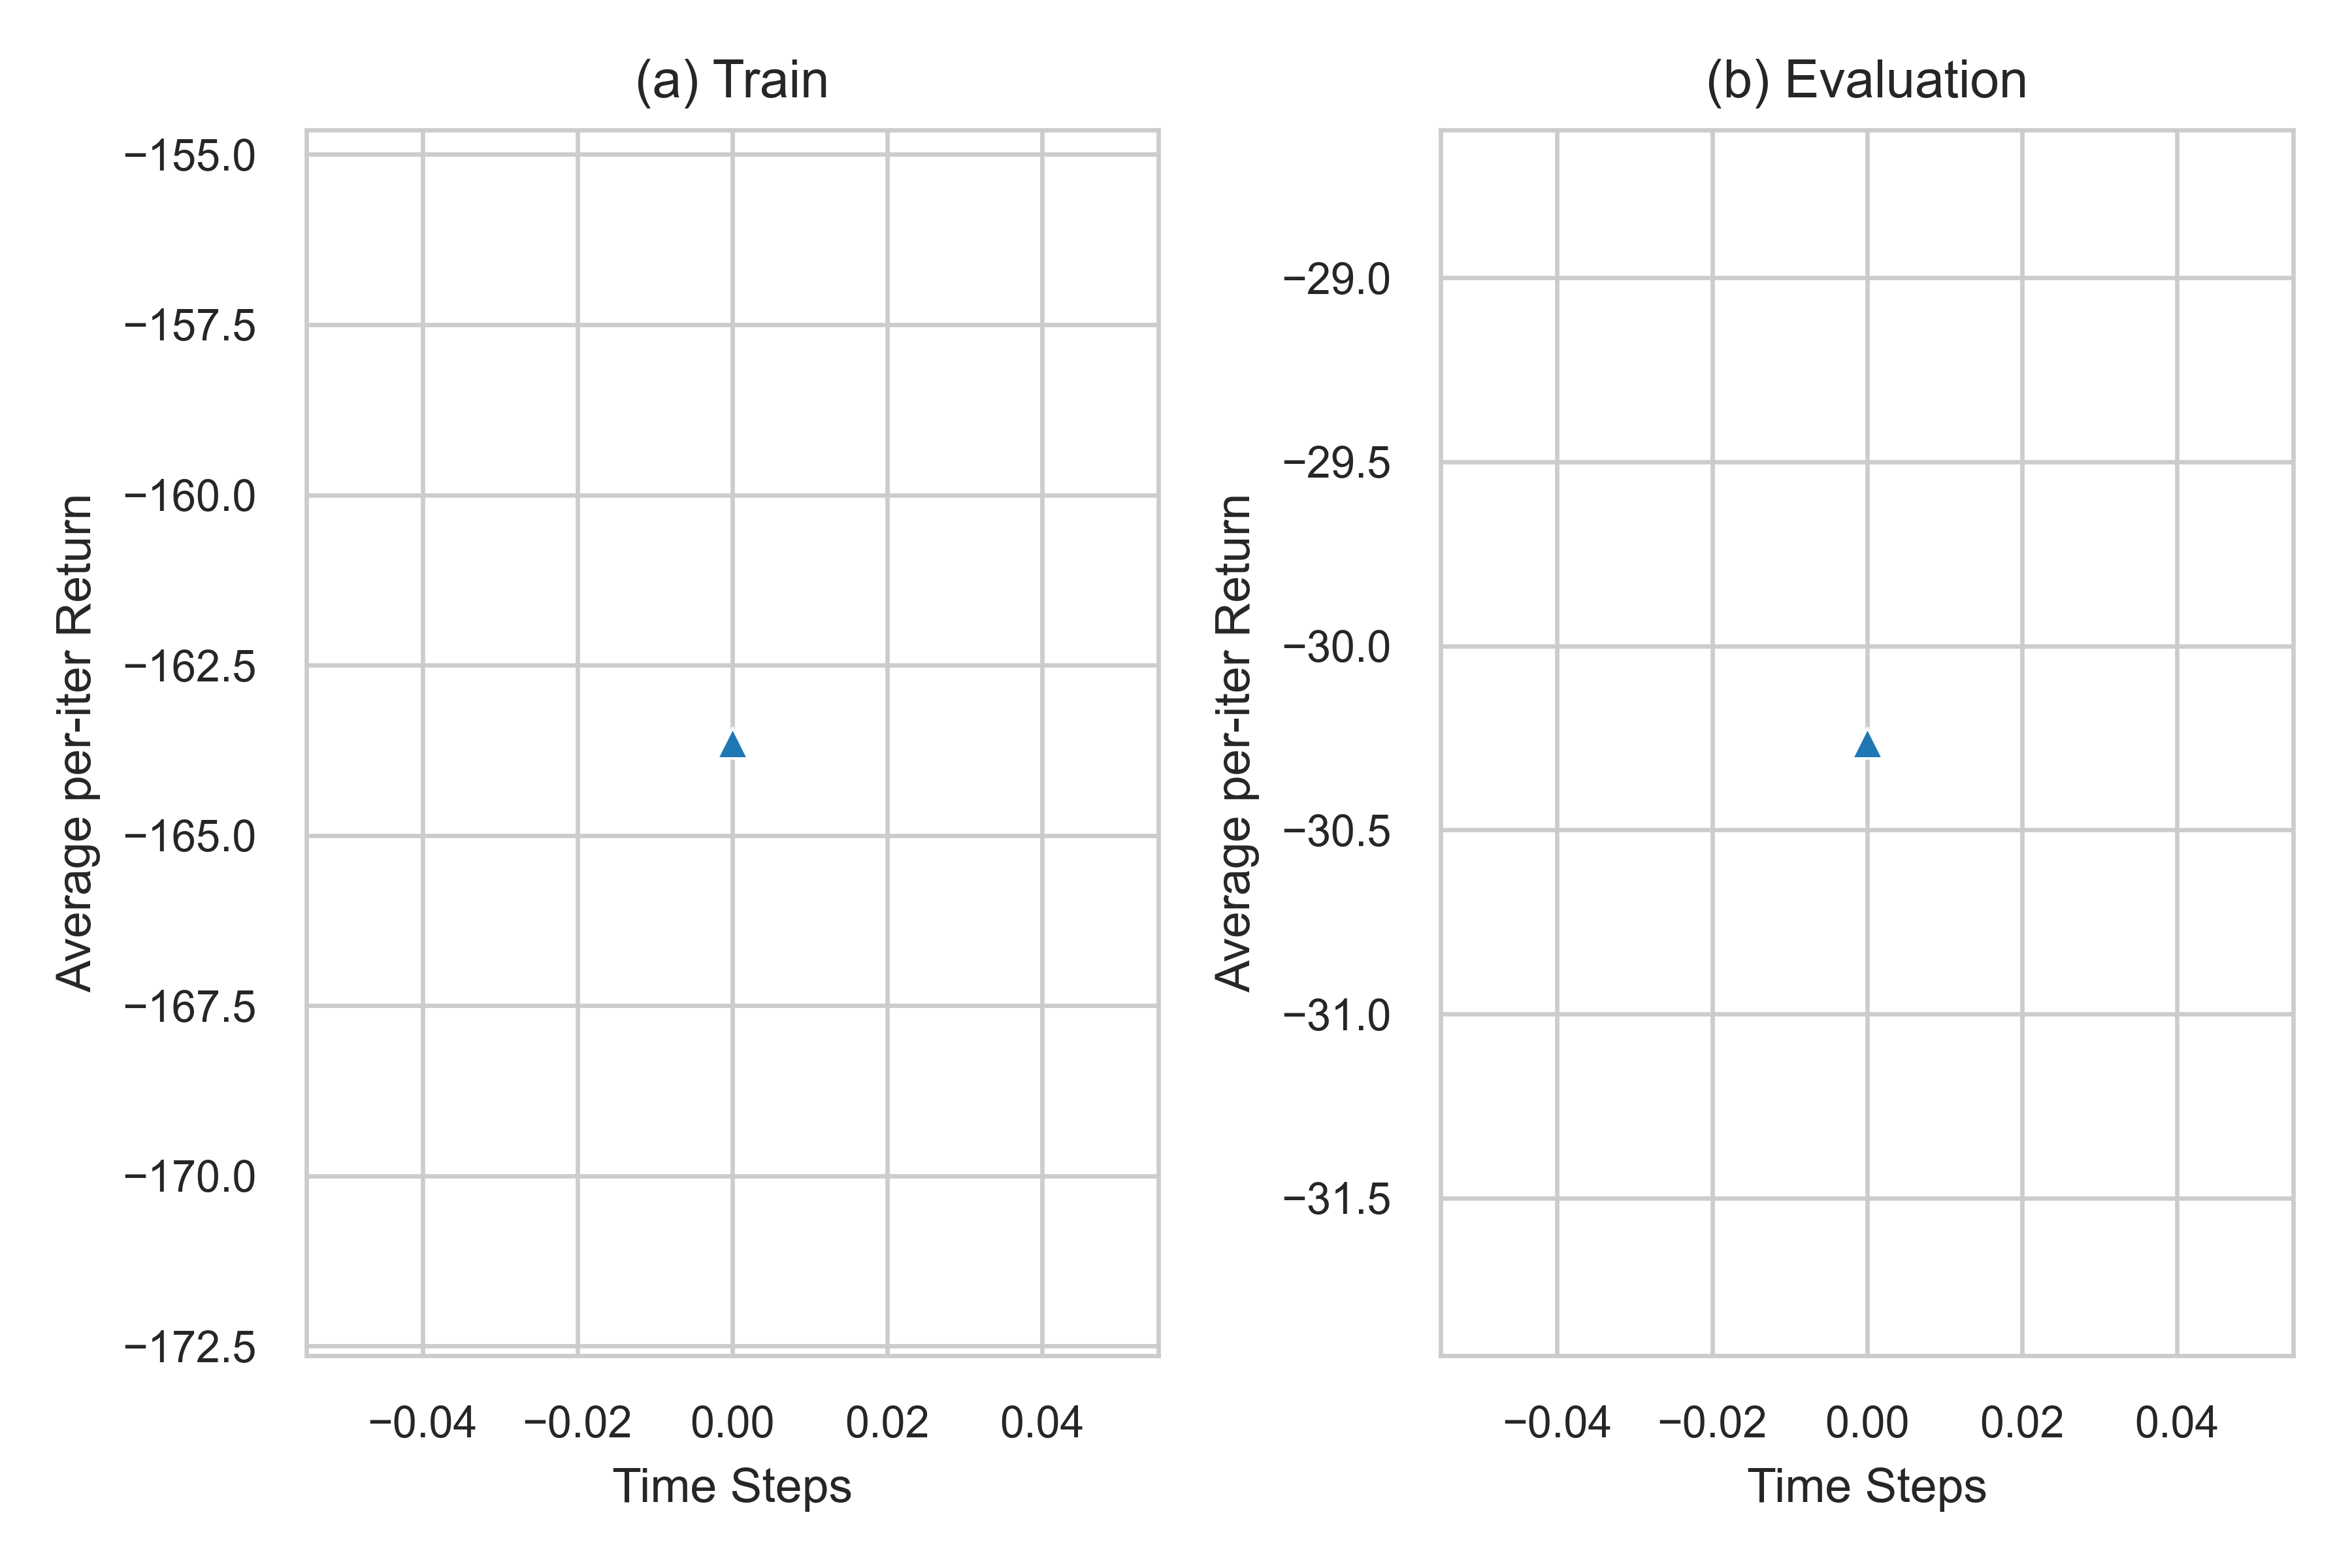
\includegraphics[width=\textwidth]{q2.png}
    \caption{Average returns in (a) training and (b) evaluation procedure. As expected, the training one is -163.6 and the evaluation one is -30.26.}
    \label{fig:2}
\end{figure}

\begin{lstlisting}
    echo "Running Homework 4 Problem 2";
    python cs285/scripts/run_hw4_mb.py --exp_name q2_obstacles_singleiteration --env_name obstacles-cs285-v0 --add_sl_noise --num_agent_train_steps_per_iter 20 --n_iter 1 --batch_size_initial 5000 --batch_size 1000 --mpc_horizon 10 --video_log_freq -1 --mpc_action_sampling_strategy random -gpu_id $1;
    echo "Done";
\end{lstlisting}

\pagebreak
% Problem 3
\section*{Problem 3}

\begin{figure}[thbp]
    \centering
    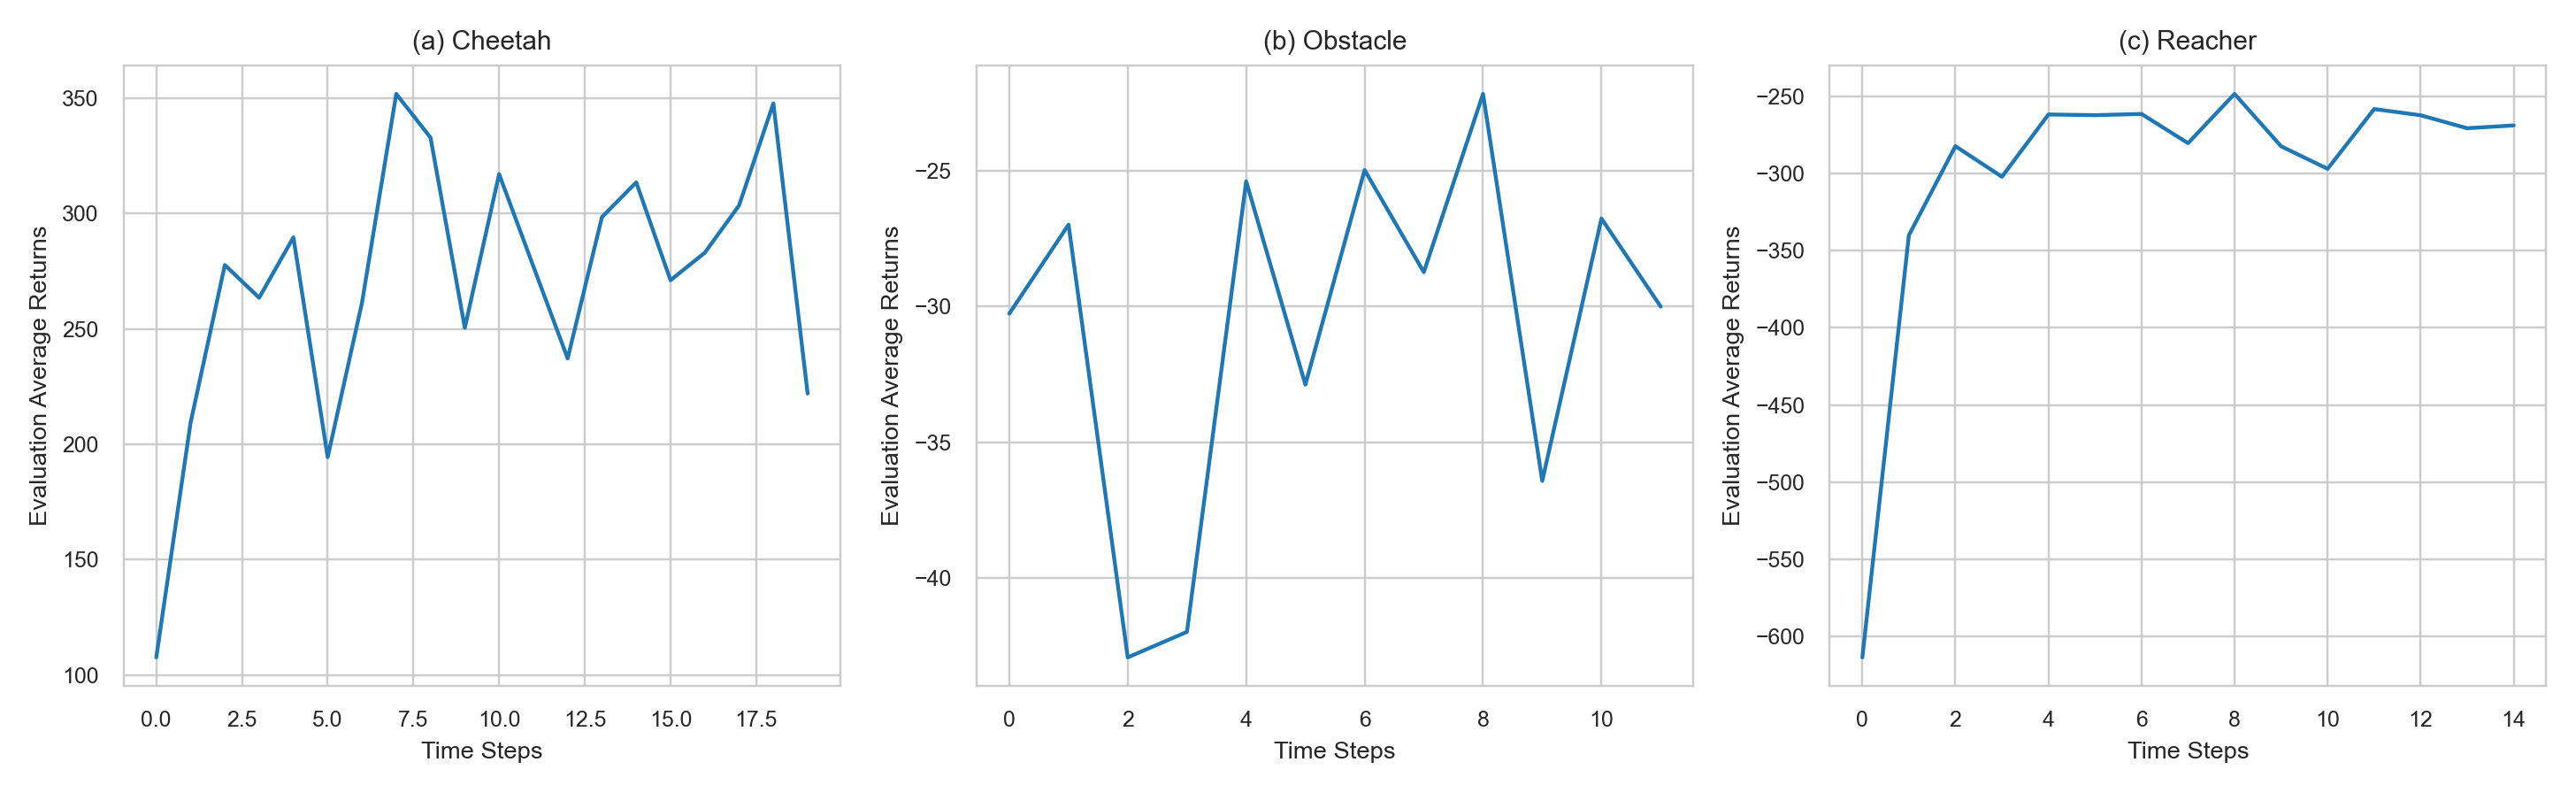
\includegraphics[width=\textwidth]{q3.png}
    \caption{Average evaluation returns in (a) Cheetah, (b) Obstacles, and (c) Reacher environments. Final values are 277.3, -30, and -268.9, respectively.}
\end{figure}

\begin{lstlisting}
    echo "Running HW4 Problem 3";
    python cs285/scripts/run_hw4_mb.py --exp_name q3_obstacles --env_name obstacles-cs285-v0 --add_sl_noise --num_agent_train_steps_per_iter 20 --batch_size_initial 5000 --batch_size 1000 --mpc_horizon 10 --n_iter 12 --video_log_freq -1 --mpc_action_sampling_strategy random -gpu_id $1 &
    python cs285/scripts/run_hw4_mb.py --exp_name q3_reacher --env_name reacher-cs285-v0 --add_sl_noise --mpc_horizon 10 --num_agent_train_steps_per_iter 1000 --batch_size_initial 5000 --batch_size 5000 --n_iter 15 --video_log_freq -1 --mpc_action_sampling_strategy random -gpu_id $1 &
    python cs285/scripts/run_hw4_mb.py --exp_name q3_cheetah --env_name cheetah-cs285-v0 --mpc_horizon 15 --add_sl_noise --num_agent_train_steps_per_iter 1500 --batch_size_initial 5000 --batch_size 5000 --n_iter 20 --video_log_freq -1 --mpc_action_sampling_strategy random -gpu_id $1 &
    wait
    echo "Done";
\end{lstlisting}

\pagebreak
% Problem 4
\section*{Problem 4}

\begin{figure}[thbp]
    \centering
    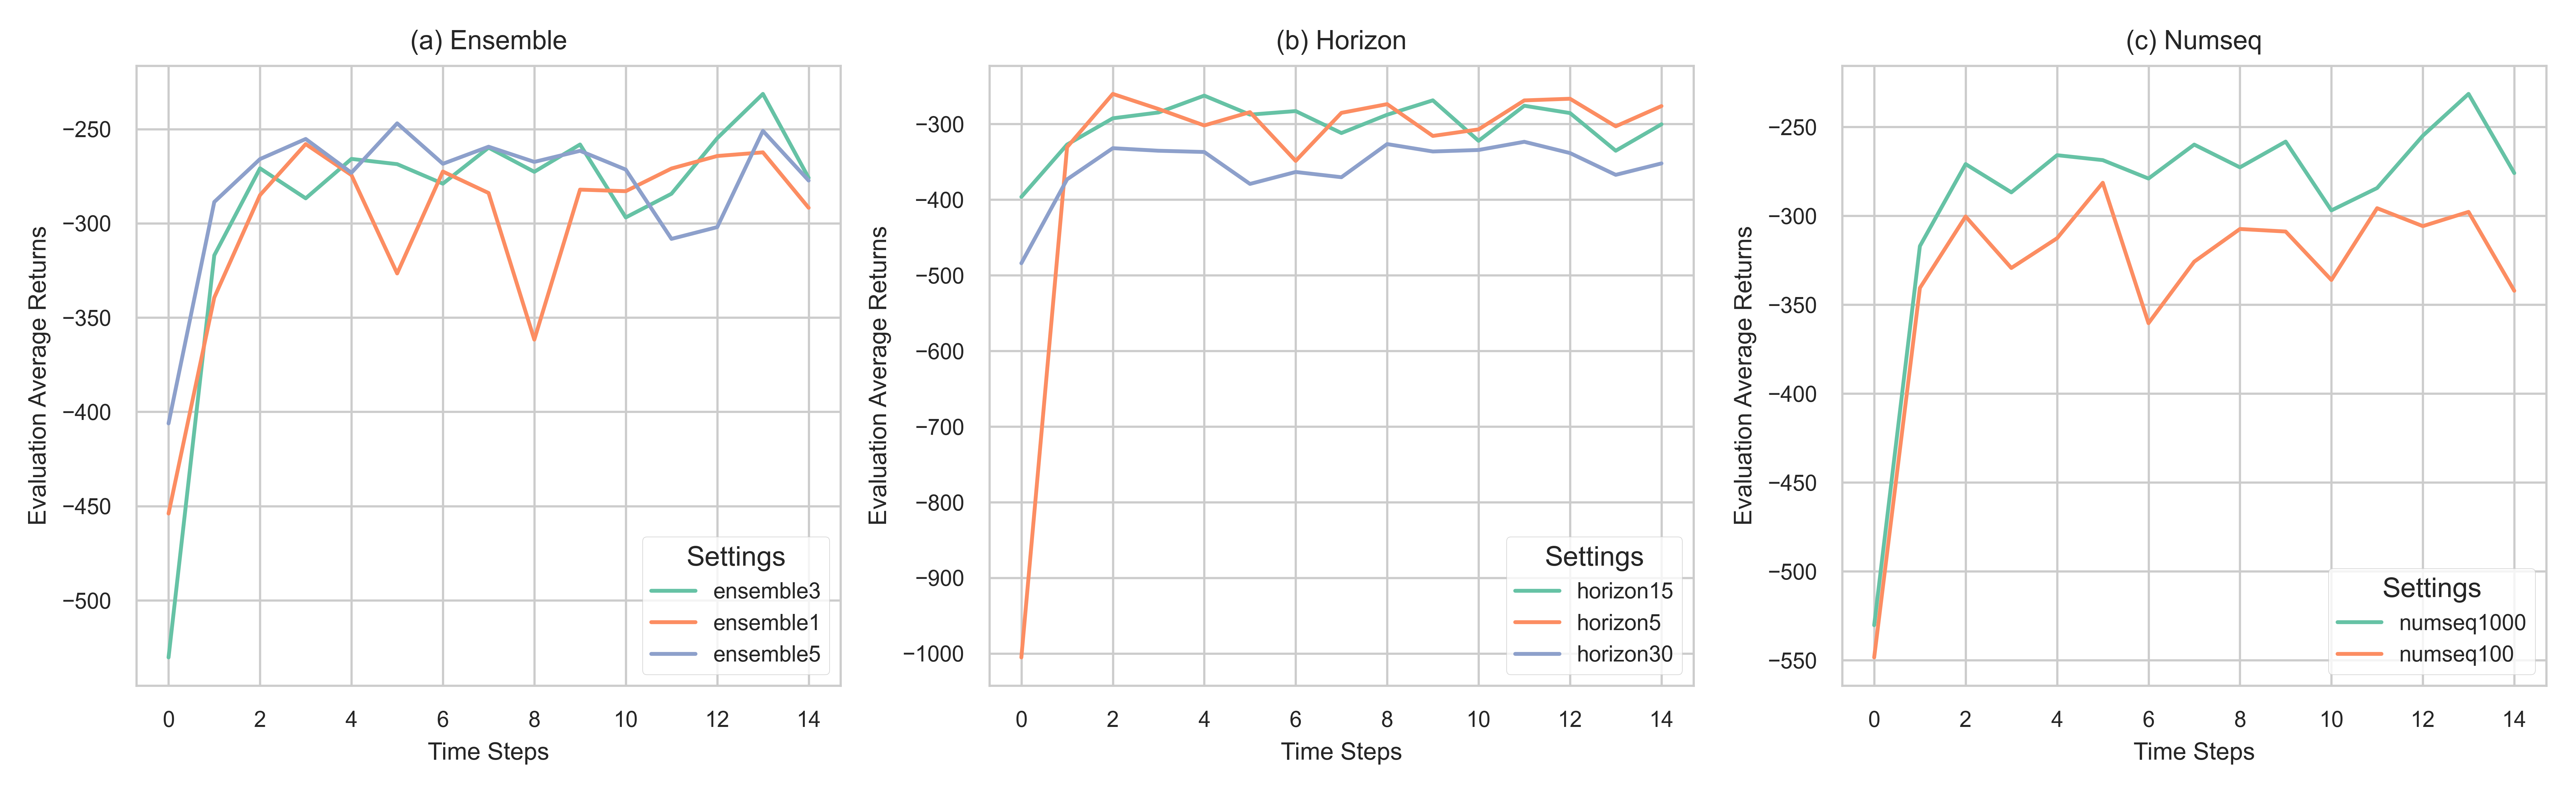
\includegraphics[width=\textwidth]{q4.png}
    \caption{Average evaluation returns with different settings of (a) number of ensemble models; (b) model predictive control horizons; and (c) number of generated action sequence.}
    \label{fig: 4}
\end{figure}

Based on the results in \hyperref[fig: 4]{Figure 4}, increasing the number of ensemble models (as shown in 4(a)) helps improve the performance but not much. Increasing prediction horizon would cause leads to higher estimation variance and prediction uncertainty, hence deteriorate the performance (as shown in 4(b)). Increasing number of generated action sequence helps explore more potential actions, which increases the possibility of achieving better score (as shown in 4(c)). 

\textbf{Codes are left out on purpose due to limited space.}

\pagebreak
% Problem 5
\section*{Problem 5}

\begin{figure}[thbp]
    \centering
    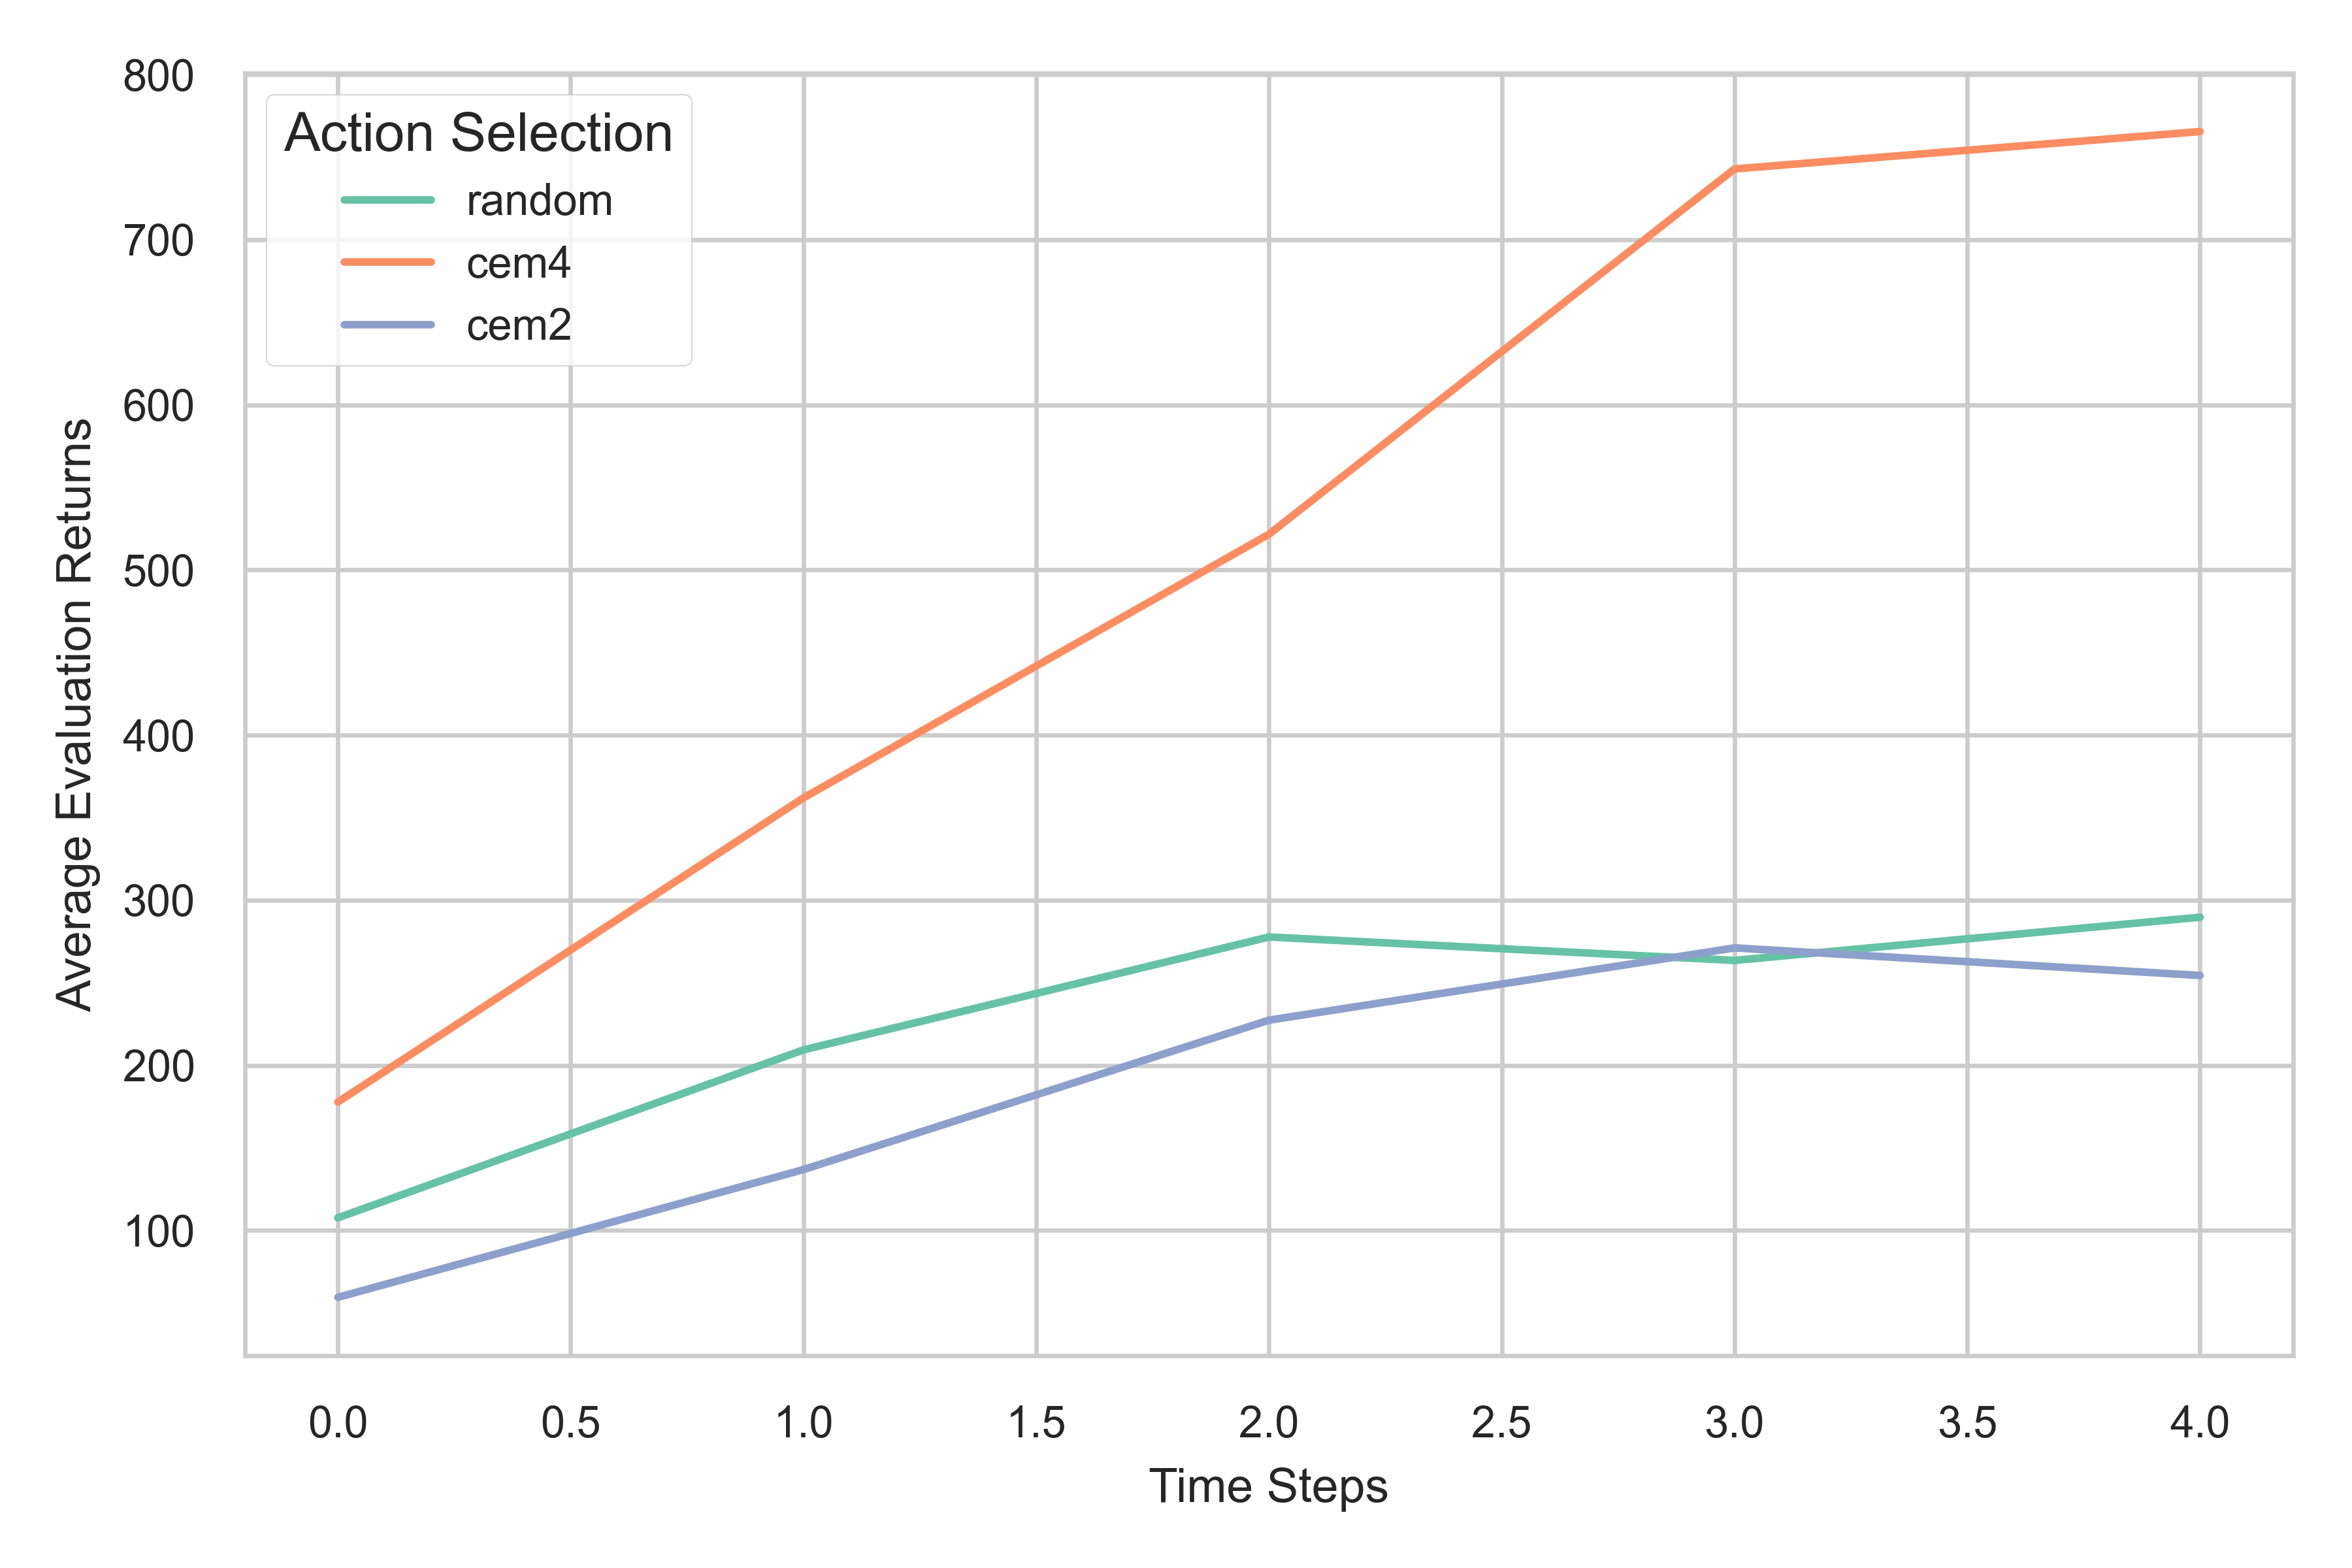
\includegraphics[width=\textwidth]{q5.png}
    \caption{Average evalutaion returns with different action selection settings. Model with 4 CEM action sampling iterations achieves the best performance at around 765.5. However, implementing 2 CEM iterations achieves lower returns than random one in my experiement. My explannation for it is that CEM performance could be affected by the initial action sequence guess. And in my case, taking only 2 CEM iterations is not sufficient to guarentee that sampled actions are the optimal.}
\end{figure}

\pagebreak
% Problem 6
\section*{Problem 6}

\end{document}